\documentclass{classrep}
\usepackage{color}
\usepackage{url}
\usepackage{hyperref}
\usepackage{amsmath}
\usepackage[T1]{fontenc}
\usepackage{polski}
\usepackage[utf8]{inputenc}
\usepackage{graphicx}
\graphicspath{ {./rys/} }

\usepackage{etoolbox}
\let\bbordermatrix\bordermatrix
\patchcmd{\bbordermatrix}{8.75}{4.75}{}{}
\patchcmd{\bbordermatrix}{\left(}{\left[}{}{}
\patchcmd{\bbordermatrix}{\right)}{\right]}{}{}

\studycycle{Informatyka, studia dzienne, I st.}
\coursesemester{VI}

\coursename{Komputerowe systemy rozpoznawania}
\courseyear{2019/2020}

\courseteacher{dr inż. Marcin Kacprowicz}
\coursegroup{poniedziałek, 12:00}

\author{
  \studentinfo{Radosław Grela}{216769} \and
  \studentinfo{Jakub Wąchała}{216914} 
}

\title{Zadanie 1: ekstrakcja cech, miary podobieństwa, klasyfikacja}


\begin{document}
\maketitle

\section{Cel} % Cel
Celem naszego zadania było stworzenie aplikacji do klasyfikacji tekstów za pomocą metody k-NN (k najbliższych sąsiadów) oraz
różnych metryk i miar podobieństwa, a następnie porównać kategorie z tymi wygenerowanymi przez aplikację.

\section{Wprowadzenie} % Wprowadzenie
Głównym zagadnieniem projektowym, z którym mieliśmy do czynienia w ramach zadania 1 była klasyfikacja statystyczna tekstów na podstawie wektora wyekstrahowanych cech. Do przeprowadzenia eksperymentu zaimplementowaliśmy algorytm \textsl{k-najbliższych sąsiadów}.

Algorytm k-najbliższych sąsiadów \textsl{(k-NN - k-nearest neighbors)} to jeden z algorytmów zaliczanych do grupy algorytmów leniwych. Jest to taka grupa algorytmów, która szuka rozwiązania dopiero, gdy pojawia się wzorzec testujący. Przechowuje wzorce uczące, a dopiero później wyznacza się odległość wzorca testowego względem wzorców treningowych. \cite{leniwy} 

Algorytm ten działa w taki sposób, że dla każdego wzorca testowego obliczana jest odległość za pomocą wybranej metryki względem wzorców treningowych, a następnie wybierana jest k najbliższych wzorców treningowych. Wynik wyznaczony jest jako najczęstszy element wśród nich. W naszym zadaniu odległość ta jest równa skali podobieństwa tekstów, a im ta odległość jest mniejsza, tym lepiej.
% cechy
%Stosunek słów kluczowych do wszystkich słów w pierwszych 10% tekstu
%Stosunek słów kluczowych do wszystkich słów w ostatnich 10% tekstu
%Stosunek słów kluczowych do wszystkich słów w dokumencie
%Stosunek słów kluczowych gdzie ilość liter (0,4] do wszystkich słów
%Stosunek słów kluczowych do wszystkich słów gdzie ilość liter słów kluczowych 8+
%Stosunek linii do ilości akapitów
%Stosunek słów o długości >6 do wszystkich słów
%Stosunek słów o długości <=6 do wszystkich słów
%Ilość słów unikalnych
%Ilość słów, których długość wynosi [5,8]
%Najczęściej występujące słowo kluczowe
\subsection{Ekstrakcja cech}
Do ekstrakcji cech charakterystycznych tekstu utworzyliśmy wektor cech, który opisuje tekst za pomocą 11 cech. Liczba słów zawsze jest liczona po zastosowaniu stop-listy oraz stemizacji, bez znaków przestankowych.
\begin{itemize}
\item[•] $C_1$ - Stosunek słów kluczowych do wszystkich słów w pierwszych 10\% tekstu. Obliczona jest za pomocą wzoru:
\begin{equation} S_{k10} = S_{10} \cap S_k  \end{equation}
\begin{equation} C_1 = \frac{|S_{k10}|}{|S_{10}|}   \end{equation} gdzie \\
$S_k$ - zbiór wszystkich słów kluczowych, \\
$S_{10}$ - zbiór słów w pierwszych 10\% tekstu, \\
$S_{k10}$ - zbiór słów kluczowych w pierwszych 10\% tekstu, \\
$|S_{k10}|$ - liczba słów kluczowych w pierwszych 10\% tekstu, \\
$|S_{10}|$ - liczba wszystkich słów w dokumencie w pierwszych 10\% tekstu. \\

\item[•] $C_2$ - Stosunek słów kluczowych do wszystkich słów w ostatnich 10\% tekstu. Obliczona jest za pomocą wzoru:
\begin{equation} S_{k90} = S_{90} \cap S_k  \end{equation}
\begin{equation} C_2 = \frac{|S_{k90}|}{|S_{90}|}   \end{equation}
 gdzie \\
$S_{90}$ - zbiór słów w ostatnich 10\% tekstu, \\
$S_{k90}$ - zbiór słów kluczowych w ostatnich 10\% tekstu, \\
$|S_{k90}|$ - liczba słów kluczowych w ostatnich 10\% tekstu, \\
$|S_{90}|$ - liczba wszystkich słów w dokumencie w ostatnich 10\% tekstu. \\

\item[•] $C_3$ - Stosunek słów kluczowych do wszystkich słów w dokumencie. Obliczona jest za pomocą wzoru:
\begin{equation} S_{k3} = S \cap S_k  \end{equation}
\begin{equation} C_3 = \frac{|S_{k3}|}{|S|}  \end{equation} gdzie \\
$S_{k3}$ - zbiór wszystkich słów kluczowych znajdujących się w dokumencie, \\
$|S_{k3}|$ - liczba wszystkich słów kluczowych znajdujących się w dokumencie, \\
$S$ - zbiór wszystkich słów w dokumencie, \\
$|S|$ - liczba wszystkich słów w dokumencie. \\

\item[•] $C_4$ - Stosunek słów kluczowych, których ilość liter $\in$ (0,4] do wszystkich słów w dokumencie. Obliczona jest za pomocą wzoru:

\begin{equation} S_{k_{4}} = S \cap S_{k_{04}}  \end{equation}
\begin{equation} C_4 = \frac{|S_{k_{4}}|}{|S|}  \end{equation} gdzie \\
$S_{k_{04}}$ - zbiór słów kluczowych, których ilość liter $\in$ (0,4], \\
$S_{k_{4}}$ - zbiór słów kluczowych znajdujących się w dokumencie, których ilość liter $\in$ (0,4], \\
$|S_{k_{4}}|$ - liczba słów kluczowych znajdujących się w dokumencie, których ilość liter $\in$ (0,4]. \\

\item[•] $C_5$ - Stosunek słów kluczowych, których ilość liter jest $\geq$8 do wszystkich słów w dokumencie. Obliczona jest za pomocą wzoru:
\begin{equation} S_{k_{5}} = S \cap S_{k_{8+}}  \end{equation}
\begin{equation} C_5 = \frac{|S_{k_{5}}|}{|S|}  \end{equation} gdzie \\
$S_{k_{8+}}$ - zbiór słów kluczowych, których ilość liter $\geq$8, \\
$S_{k_{5}}$ - zbiór słów kluczowych znajdujących się w dokumencie, których ilość liter $\geq$8, \\
$|S_{k_{5}}|$ - liczba słów kluczowych znajdujących się w dokumencie, których ilość liter $\geq$8. \\

\item[•] $C_6$ - Stosunek linii do ilości akapitów. Obliczona jest za pomocą wzoru:
\begin{equation} C_{6} = \frac{|l|}{|a|}  \end{equation} gdzie \\
$|l|$ - liczba linii,\\
$|a|$ - liczba akapitów.\\
Na rysunku \ref{c6png} został zamieszczony przykładowy artykuł. Dla tego przykładu, $|l| = 24$, a $|a| = 8$. \\
\begin{figure}[h!]
	\centering
	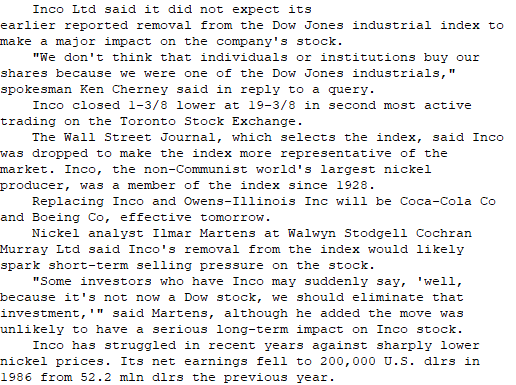
\includegraphics[width=0.6\textwidth]{c6.png}
	\caption{Przykładowy artykuł.}
	\label{c6png}
\end{figure}

\item[•] $C_7$ - Stosunek słów, których ilość liter jest większa niż 6 do wszystkich słów w dokumencie. Obliczona jest za pomocą wzoru:
\begin{equation} C_7 = \frac{|S_{k_{6+}}|}{|S|}  \end{equation} gdzie \\
$S_{k_{6+}}$ - zbiór słów w dokumencie, których ilość liter jest większa niż 6, \\
$|S_{k_{6+}}|$ - liczba słów w dokumencie, których ilość liter jest większa niż 6. \\

\item[•] $C_8$ - Stosunek słów, których ilość liter jest $\leq$6 do wszystkich słów w dokumencie. Obliczona jest za pomocą wzoru:
\begin{equation} C_8 = \frac{|S_{k_{06}}|}{|S|}  \end{equation} gdzie \\
$S_{k_{06}}$ - zbiór słów w dokumencie, których ilość liter jest $\leq$ 6, \\
$|S_{k_{06}}|$ - liczba słów w dokumencie, których ilość liter jest $\leq$ 6. \\

\item[•] $C_9$ - Ilość słów unikalnych. Jest to liczba słów, które wystąpiły w tekście co najmniej raz. Przykładowo, dla zdania \textsl{,,Być albo nie być''} ilość słów unikalnych jest równa 3 (\textsl{być, albo, nie}).\\

\item[•] $C_{10}$ - Ilość słów w dokumencie, których ilość liter $\in$ [5,8]. Pseudokod obliczający wartość cechy $C_{10}$:
\textsl{
\begin{itemize}
\item $C_{10}$=0
\item Dla każdego słowa w artykule:
	\begin{itemize}
	\item Jeżeli długość słowa $\geq$5 i długość słowa $\leq$8:
		\begin{itemize}
		\item $C_{10}$++;
		\end{itemize}
	\end{itemize}
\item Zwróć $C_{10}$
\end{itemize}
} 


\item[•] $C_{11}$ - Najczęściej występujące słowo kluczowe. Przykładowo, dla tekstu na rysunku \ref{c6png} i zbioru słów kluczowych \textsl{\{Inco, pressure, against, year\}} najczęściej występującym słowem kluczowych jest słowo \textsl{Inco}. Jest to cecha tekstowa, której podobieństwo z innym słowem mierzymy jedną z dwóch miar podobieństwa ciągów znaków opisanych w sekcji \textsl{Metryki i miary podobieństwa}.
\end{itemize}

%Czy np. im tekst dłuższy, tym bardziej związany z etykietą USA lub CANADA? (istotne!)}

\subsection{Wyznaczanie słów kluczowych}
Wyznaczenie słów kluczowych przebiega w następujący sposób: na początek za pomocą klasy WordCounter zliczane są wszystkie słowa w artykułach oraz jednocześnie dodawane do odpowiednich list w tej klasie. Każda zmienna jest listą stringów o nazwie wordCountDictionary + nazwa kraju. Dodatkowo, przechowywany jest słownik typu \textsl{<string, int>}, którego kluczem jest słowo, a wartość to ilość wystąpień tego słowa we wszystkich artykułach. Po podliczeniu wszystkich słów oraz przydzieleniu do odpowiednich list wybieramy po 18 najpopularniejszych słów dla każdego kraju, które występują tylko w tym jednym konkretnym kraju. Na koniec $18*6 = 108$ słów zostaje słowami kluczowymi. Cały proces wyznaczania słów kluczoywch jest dokonywany po zastosowaniu stop-listy oraz po stemizacji. Ponadto, proces wybierania słów kluczowych pomija 20\% wszystkich podliczonych słów, aby proces dopasowywania słów kluczowych do krajów nie trwał zbyt długo.
\subsection{Metryki i miary podobieństwa}
Do liczenia odległości pomiędzy artykułami oraz obliczenia miary podobieństwa używaliśmy 3 metryk i 2 miar podobieństwa ciągów tekstowych.
\begin{enumerate}
\item Metryka Euklidesowa - aby obliczyć odległość $d_e(x,y)$ między wektorami x i y należy obliczyć pierwiastek kwadratowy z sumy kwadratów różnic wartości współrzędnych wektora o tych samych indeksach. Wzór jest następujący \cite{euc}:
\begin{equation} 
d_e(x,y)=\sqrt{(x_1-y_1)^2+\ldots+(x_n-y_n)^2}
\end{equation} gdzie $x_i$ i $y_i$ to cechy wektora.
\item Metryka uliczna - odległość $d_m(x,y)$ jest równa sumie wartości bezwzględnych z różnic wartości współrzędnych wektora o tych samych indeksach \cite{manh}:
\begin{equation} 
d_m(x,y)=\sum_{n=1}^{N} |{x_n-y_n}|
\end{equation} gdzie $x_i$ i $y_i$ to cechy wektora.
\item Metryka Czebyszewa - odległość $d_c(x,y)$ w tej metryce jest równa maksymalnej wartości bezwględnych różnic współrzędnych punktów x oraz y, zgodnie ze wzorem \cite{cze}:
\begin{equation} 
d_c(x,y)=\max_{i} |{x_i-y_i}|
\end{equation} gdzie $x_i$ i $y_i$ to cechy wektora.
\item Miara \textsl{n}-gramów - metoda ta określa podobieństwo łańcuchów tekstowych $s_1$, $s_2$ w oparciu o ilość wspólnych podciągów n-elementowych, czyli \textsl{n}-gramów \cite{wyklad}:
\begin{equation}
sim_n(s_1, s_2) = \frac{1}{N-n+1} \sum_{i=1}^{N-n+1} h(i)
\end{equation} gdzie 

$h(i) = 1$, jeśli n-elementowy podciąg zaczynający się od i-tej pozycji w $s_1$ występuje co najmniej raz w  $s_2$, w przeciwnym razie $h(i) = 0$

$N-n+1$ - ilość możliwych n-elemenetowych podciągów w $s_1$.

W naszym programie n jest stałe i wynosi 3.
\item Uogólniona miara \textsl{n-gramów} (Miara Niewiadomskiego) - ta miara jest ulepszoną wersją miary n-gramów. Bada ona podobieństwo poprzez sprawdzenie podciągów różnej długości od jedno- do N-elementowych, gdzie N jest długością słowa  \cite{wyklad}:
\begin{equation}
\mu_N(s_1, s_2) = \frac{2}{N^2+N} \sum_{i=1}^{N(s_1)} \sum_{j=1}^{N(s_1)-i+1} h(i,j)
\end{equation} gdzie

$h(i,j) = 1$, jeśli $i$-elementowy podciąg w słowie $s_1$ zaczynający się od $j$-tej pozycji w słowie $s_1$ pojawia się co najmniej raz w  słowie $s_2$, w przeciwnym razie $h(i,j) = 0$,

$N(s_1), N(s_2)$ – ilość liter w słowach $s_1$ i $s_2$,

$N = max\{(s_1), N(s_2)\}$,

$\frac{N^2+N}{2}$ - ilość możliwych podciągów od 1-elementowych do $N$-elementowych w słowie o długości $N$.
\end{enumerate}

Aby porównać wektory za pomocą metryk w algorytmie k-NN, najpierw wyznaczamy miarę podobieństwa z ostatniej, 11 cechy, która jest cechą tekstową. Wyznaczamy ją za pomocą jednej z dwóch miar. Ponieważ w tych miarach im bliżej 1, tym lepiej, odejmujemy tą liczbę od 1, a następnie używamy jej w metryce.
%\item Miara \textsl{Term Frequency Matrix}, czyli po polsku ,,macierz częstości występowania terminów'' podaje wartość podobieństwa dokumentów $d_1$ i $d_2$ ze względu na wybrany %zbiór terminów, np. słów kluczowych. Ustawiamy macierz słów kluczowych i dokumentów:
%\begin{equation}
%\bbordermatrix{~ & t_1 & t_2 & \ldots & t_n \cr
        %          d_1 & a_{11} & a_{12} & \ldots & a_{1n} \cr
    %              d_2 & a_{21} & a_{22} & \ldots & a_{2n} \cr}
%\end{equation}
%Następnie podobieństwo otrzymanych wektorów jest obliczone przy pomocy amplitudy kosinusowej: 
%\begin{equation}
%r_{ca}(V_1, V_2)= \textsl{$\frac{|\sum_{i=1}^{n} a_{1i}*a_{2i}|}{\sqrt{\sum_{i=1}^{n} a_{1i}^2 * \sum_{i=1}^{n} a_{2i}^2}}$}
%\end{equation}

\subsection{Miary jakości}
W wynikach klasyfikacji używamy następujących miar jakości \cite{apr}:
\begin{itemize}
\item[•] Accuracy:
\begin{equation}
ACC = \frac{TP + TN}{TP + TN + FP + FN}
\end{equation}
\item[•] Precision
\begin{equation}
PPV = \frac{TP}{TP + FP}
\end{equation}
\item[•] Recall
\begin{equation}
TPR = \frac{TP}{TP + FN}
\end{equation}
\end{itemize}
Oznaczenia użytych symboli:

TP - miara prawdziwie pozytywna (\textsl{true positive}), czyli poprawnie zaklasyfikowane artykuły dla badanej etykiety 

TN - miara prawdziwie negatywna (\textsl{true negative}), czyli poprawnie zaklasyfikowane artykuły dla pozostałych etykiet

FP - miara fałszywie pozytywna (\textsl{false positive}), czyli niepoprawnie zaklasyfikowane artykuły dla badanej etykiety 

FN - miara fałszywie negatywna (\textsl{false negative}), czyli niepoprawnie zaklasyfikowane artykuły dla pozostałych etykiet

\subsection{Normalizacja wektorów cech}
Wszystkie wartości wektora cech zostaną znormalizowane za pomocą wzoru (\ref{norm_}) \cite{norm}:
\begin{equation} \label{norm_} x_{scaled} = \frac{x - x_{min}}{x_{max} - x_{min}}  \end{equation}
Dzięki temu, wektor będzie zawierał tylko wartości z przedziału $[0,1]$.
\section{Opis implementacji} % Opis implementacji
Nasza aplikacja została utworzona w języku C\# i jest to aplikacja konsolowa. Poniżej opisane zostały wszystkie klasy oraz dane zawarte w naszym projekcie:
\begin{itemize}
\item Klasa Program to klasa główna naszego programu. Jest swego rodzaju kontrolerem dla pozostałych klas. Znajduje się tutaj funkcja \textsl{main}, która rozpoczyna wykonywanie programu.
\item W katalogu \textsl{dane} znajdują się wszystkie pliki z artyukłami, które są wykorzystywane do badań.
\item Klasa Metric jest klasą abstrakcyjną. Odpowiada za obliczenia odległości tekstów. Po tej klasie dziedziczą klasy: EuclideanMetric, ChebyshewMetric oraz ManhattanMetric.
\item Klasa Measure jest klasą abstrakcyjną. Po niej dziedziczą klasy \textsl{GeneralizedNGramsMeasure} i \textsl{NGramsMeasure}, które odpowiadają za obliczanie miar podobieństwa łańcuchów tekstowych.
\item Klasa Feature jest klasą abstrakcyjną. Po niej dziedziczy 10 klas: Feature 1-10, które reprezentują każdą z 10 wyekstrahowanych przez nas cech.
\item Klasa Stemmer to klasa, która odpowiada za stemizację tekstów. Została ona zapożyczona z \cite{stemmer}
\item Klasa StopwordTool jest klasą odpowiedzialną za usuwanie słów znajdujących się na stopliście. Również została znaleziona i zapożyczona z Internetu ze strony \cite{stopword}
\item WordCounter jest używany do zliczania słów wszystkich artykułów i podania ich liczności. Potrzebny głównie do  wyznaczenia słów kluczowych.
\item Klasa KeyWords odpowiada za wyznaczenie 100 słów kluczowych. Metoda wyznaczania słów kluczowych została opisana w sekcji 2.
\item Klasa FileReader odpowiada za otwieranie każdego pliku z artykułami
\item FileParser to klasa odpowiedzialna za parsowanie danych z konkretnego pliku.
\item Article to klasa reprezentująca artykuł. Zawiera takie cechy jak: tekst oryginalny, tekst przetworzony, \textsl{place}, \textsl{classifiedPlace}, wektor cech.
\item Klasa Neighbor to klasa, która przechowuje artykuł oraz obliczoną wartość algorytmu k-NN dla konkretnego, obecnie sprawdzanego artykułu w algorytmie. Wykorzystujemy ją, aby znaleźć najbliższych k sąsiadów.
\item KNN to klasa odpowiedzialna za algorytm k najbliższych sąsiadów. 
\end{itemize}
Na rysunku \ref{exampleRun} przedstawiony został wynik z konsoli po przykładowym uruchomieniu programu, natomiast na rysunku \ref{uml} przedstawiony został diagram UML naszego programu. 


% ????????????????????????????????
\begin{figure}[h!]
	\centering
	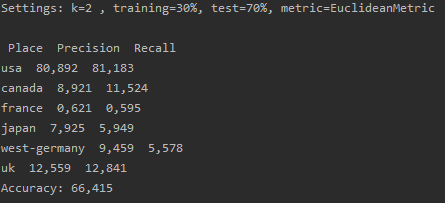
\includegraphics[width=0.4\textwidth]{exampleRun.png}
	\caption{Wynik z przykładowego uruchomienia programu.}
	\label{exampleRun}
\end{figure}
% ????????????????????????????????

\begin{figure}[h!]
	\centering
	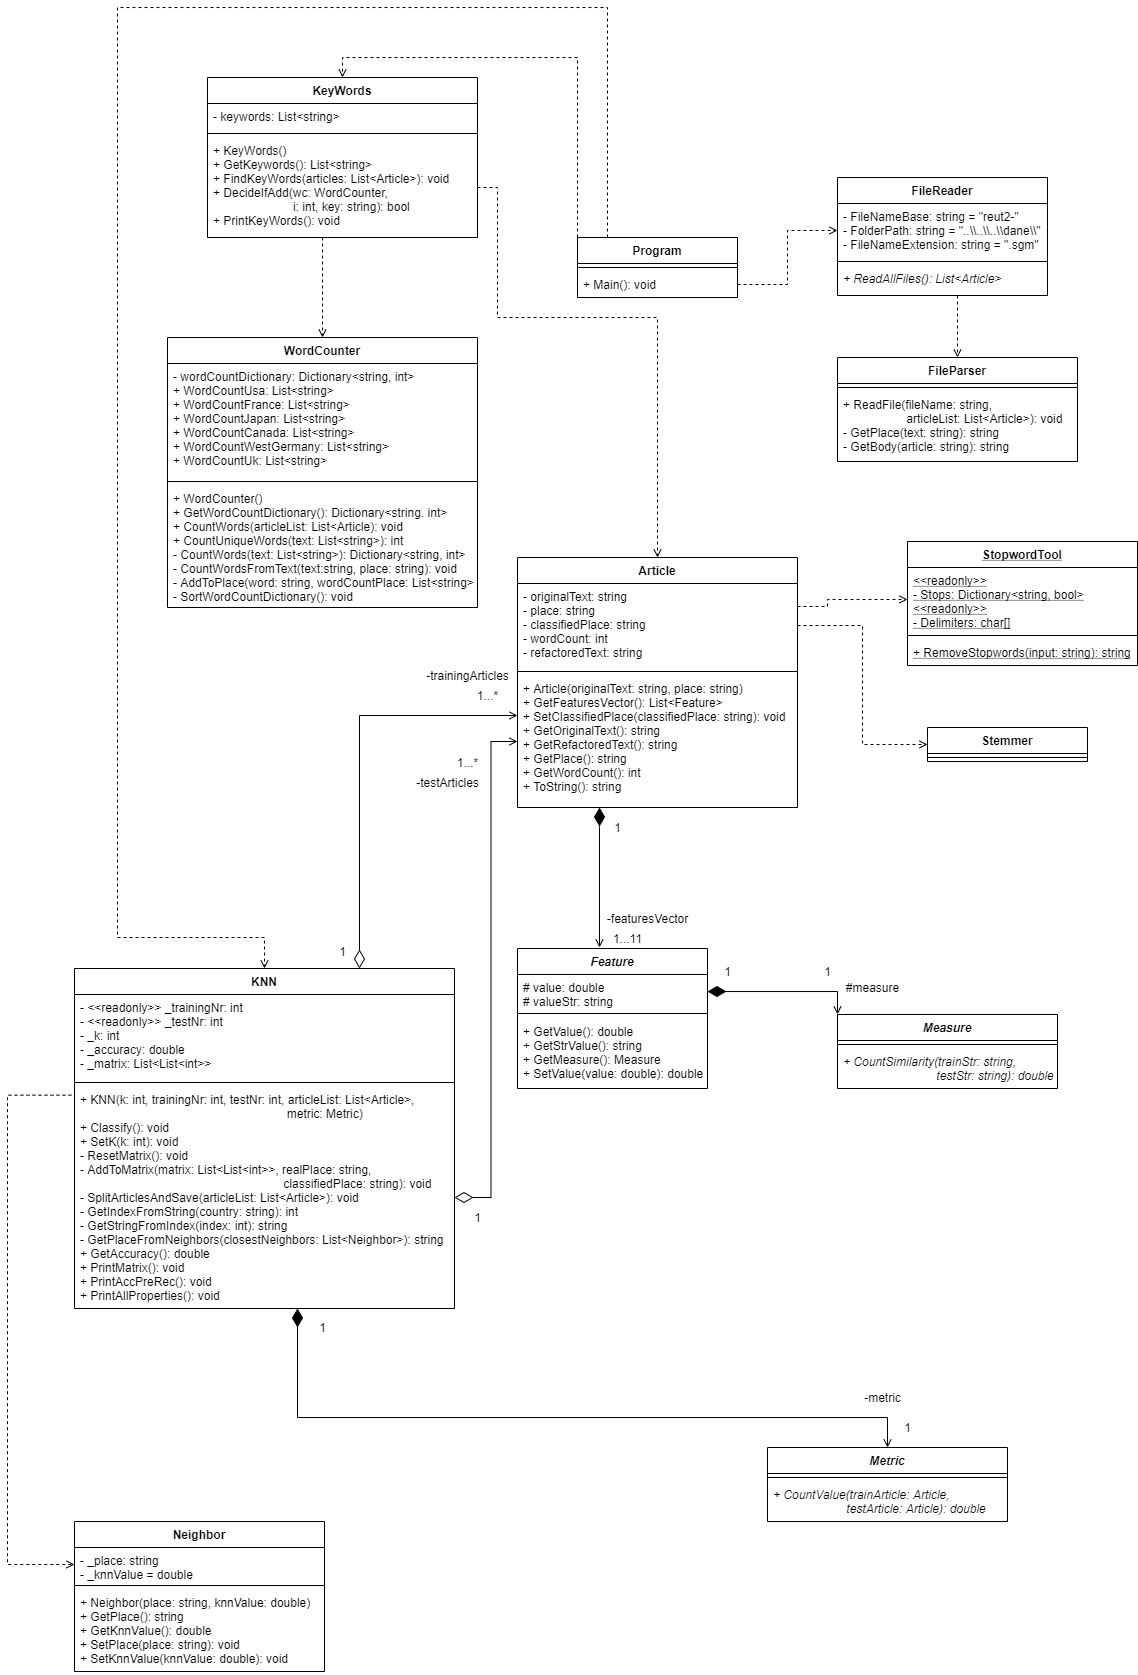
\includegraphics[width=1\textwidth]{uml.png}
	\caption{Diagram UML.}
	\label{uml}
\end{figure}


\newpage
\section{Materiały i metody} % Materiały i metody
Wykonana przez nas klasyfikacja została wykonana za pomocą wszystkich trzech metryk oraz dwóch miar podobieństwa. Każdy przypadek testowy był klasyfikowany dla dziesięciu różnych wartości k najbliższych sąsiadów: 2, 3, 4, 5, 7, 10, 13, 15, 20, 25.

Klasyfikacji dokonywaliśmy tylko na tych tekstach, które miały jedną z etykiet: \textsl{west-germany, usa, france, uk, canada, japan} i były to ich jedyne etykiety.

Dokonaliśmy pięciu różnych podziałów na dane testowe oraz treningowe:
\begin{itemize}
\item 30\% dane treningowe, 70\% dane testowe
\item 50\% dane treningowe, 50\% dane testowe
\item 70\% dane treningowe, 30\% dane testowe
\item 80\% dane treningowe, 20\% dane testowe
\item 85\% dane treningowe, 15\% dane testowe
\end{itemize}

Poniżej zostały opisane 4 wykonane przez nas eksperymenty.

\subsection{Badanie zależności Accuracy od parametru k}

W tym eksperymencie badaliśmy wpływ doboru parametru k na Accuracy. Program został uruchomiony dla 10 różnych wartości $k\in$ \{2, 3, 4, 5, 7, 10, 13, 15, 20, 25\}.

Klasyfikacja tekstów została wykonana dla stałej wartości podziału zbioru cech na testowe i treningowe. Był to podział 50\% dane treningowe, 50\% dane testowe.

Metryką, jakiej użyliśmy była metryka euklidesowa.

\subsection{Badanie wyników klasyfikacji w zależności od wartości proporcji podziału zbioru}

W tym eksperymencie badaliśmy wpływ wartości proporcji podziału zbioru na Accuracy. Program został uruchomiony dla k=10.

Badane podziały były następujące:
\begin{itemize}
	\item 30\% dane treningowe, 70\% dane testowe
	\item 50\% dane treningowe, 50\% dane testowe
	\item 70\% dane treningowe, 30\% dane testowe
	\item 80\% dane treningowe, 20\% dane testowe
	\item 85\% dane treningowe, 15\% dane testowe
\end{itemize}

Metryką, jakiej użyliśmy była metryka uliczna.

\subsection{Badanie zależności Accuracy od wyboru metryki}

W tym eksperymencie badaliśmy zależność Accuracy od wyboru metryki. Program został uruchomiony dla k=13. Podział na dane treningowe i testowe był stały i wynosił 70\% treningowe i 30\% testowe.

\subsection{Badanie zależności Accuracy od wyboru podzbioru cech}

W tym eksperymencie badaliśmy zależność Accuracy od wyboru podzbioru cech. Program został uruchomiony dla k=20. Metryka, jakiej użyliśmy to metryka Czebyszewa. Podział na dane treningowe i testowe był stały i wynosił 50\% treningowe i 50\% testowe. Podzbiory cech jakie badaliśmy były następujące:
\begin{itemize}
	\item Wszystkie cechy
	\item $C_1, C_2, C_3, C_4, C_5, C_{11}$
	\item $C_6, C_7, C_8, C_9, C_{10}$ 
	\item $C_1, C_2, C_3, C_8, C_9, C_{10}$
	\item $C_4, C_5, C_6, C_7, C_{11}$
\end{itemize}


\section{Wyniki} % Wyniki
\subsection{Wartości wektorów cech przed normalizacją}
\begin{itemize}
	\item Cecha $C_{1}$ zawierała się w wartościach $\in [0,1]$
	\item Cecha $C_{2}$ zawierała się w wartościach $\in [0,0.5]$
	\item Cecha $C_{3}$ zawierała się w wartościach $\in [0,0.155]$
	\item Cecha $C_{4}$ zawierała się w wartościach $\in [0,0.075]$
	\item Cecha $C_{5}$ zawierała się w wartościach $\in [0,0.1]$
	\item Cecha $C_{6}$ zawierała się w wartościach $\in [1,14]$
	\item Cecha $C_{7}$ zawierała się w wartościach $\in [0,0.591]$
	\item Cecha $C_{8}$ zawierała się w wartościach $\in [0.409,1]$
	\item Cecha $C_{9}$ zawierała się w wartościach $\in [1,420]$
	\item Cecha $C_{10}$ zawierała się w wartościach $\in [1,574]$
	\item Cecha $C_{11}$ jest cechą tekstową i nie trzeba jej było normalizować, gdyż po użyciu miary $n$-gramów przyjmuje wartości $[0,1]$.
\end{itemize}


\newpage
\subsection{Badanie wyników klasyfikacji w zależności od parametru k}
\begin{table}[h!]
	\centering
	\begin{tabular} {c c c c c c}
		\hline
		\textbf{Parametr k} & \textbf{Accuracy [\%]} & \vline & \textbf{Place} & \textbf{Precision [\%]} & \textbf{Recall [\%]}\\ [0.5ex] 
		\hline
		\hline 
		&   		&\vline& USA & 81,637 & 81,394 \\
		&			&\vline& CAN & 8,952 & 10,733 \\
		2 & 67,705	&\vline& FRA & 6,400 & 6,957 \\
		&			&\vline& JAP & 11,828 & 7,801 \\
		&			&\vline& W-G & 13,821 & 9,714 \\
		&			&\vline& UK  & 14,021 & 16,708 \\
		\hline 
		&   		&\vline& USA & 81,271 & 90,093 \\
		&			&\vline& CAN & 8,108 & 4,712 \\
		3 & 73,921	&\vline& FRA & 11,321 & 5,217 \\
		&			&\vline& JAP & 13,333 & 6,383 \\
		&			&\vline& W-G & 17,284 & 8,000 \\
		&			&\vline& UK  & 17,483 & 12,285 \\
		\hline 
		&   		&\vline& USA & 80,895 & 92,398 \\
		&			&\vline& CAN & 13,939 & 6,021 \\
		4 & 74,900 	&\vline& FRA & 14,706 & 4,348 \\
		&			&\vline& JAP & 8,000 & 3,546 \\
		&			&\vline& W-G & 20,000 & 4,571 \\
		&			&\vline& UK  & 15,086 & 8,600 \\
		\hline 
		&   		&\vline& USA & 80,703 & 94,684 \\
		&			&\vline& CAN & 13,265 & 3,403 \\
		5 & 76,799 	&\vline& FRA & 15,385 & 3,478 \\
		&			&\vline& JAP & 8,642 & 2,482 \\
		&			&\vline& W-G & 34,211 & 7,429 \\
		&			&\vline& UK  & 17,742 & 8,108 \\
		\hline 
		&   		&\vline& USA & 80,236 & 97,342 \\
		&			&\vline& CAN & 15,686 & 2,094 \\
		7 & 78,312 	&\vline& FRA & 50,000 & 1,739 \\
		&			&\vline& JAP & 10,000 & 1,064 \\
		&			&\vline& W-G & 18,750 & 1,714 \\
		&			&\vline& UK  & 23,009 & 6,388 \\
		\hline 
		&   		&\vline& USA & 79,897 & 98,401 \\
		&			&\vline& CAN & 16,129 & 1,309 \\
		10 & 79,024 &\vline& FRA & 100,000 & 0,870 \\
		&			&\vline& JAP & 5,000 & 0,355 \\
		&			&\vline& W-G & 0,000 & 0,000 \\
		&			&\vline& UK  & 7,937 & 1,229 \\

		\hline
	\end{tabular}
	\caption{Zależność Accuracy od wartości k. }
	\label{tabelaK}
\end{table}


\begin{table}[h!]
	\centering
	\begin{tabular} {c c c c c c}
		\hline
		\textbf{Parametr k} & \textbf{Accuracy [\%]} & \vline & \textbf{Place} & \textbf{Precision [\%]} & \textbf{Recall [\%]}\\ [0.5ex] 
		\hline	
		\hline 
		&   		&\vline& USA & 79,844 & 99,257 \\
		&			&\vline& CAN & 19,048 & 1,047 \\
		13 & 79,365 &\vline& FRA & 0,000 & 0,000 \\
		&			&\vline& JAP & 0,000 & 0,000 \\
		&			&\vline& W-G & 0,000 & 0,000 \\
		&			&\vline& UK  & 16,000 & 0,983 \\
		\hline 
		&   		&\vline& USA & 79,899 & 99,517 \\
		&			&\vline& CAN & 22,222 & 1,047 \\
		15 & 79,410	&\vline& FRA & 0,000 & 0,000 \\
		&			&\vline& JAP & 0,000 & 0,000 \\
		&			&\vline& W-G & 0,000 & 0,000 \\
		&			&\vline& UK  & 27,778 & 1,229 \\
		\hline 
		&   		&\vline& USA & 79,807 & 99,684 \\
		&			&\vline& CAN & 18,750 & 0,785 \\
		20 & 79,632 &\vline& FRA & 0,000 & 0,000 \\
		&			&\vline& JAP & 0,000 & 0,000 \\
		&			&\vline& W-G & 0,000 & 0,000 \\
		&			&\vline& UK  & 0,000 & 0,000 \\
		\hline 
		&   		&\vline& USA & 79,828 & 99,814 \\
		&			&\vline& CAN & 25,000 & 0,785 \\
		25 & 79,795 &\vline& FRA & 0,000 & 0,000 \\
		&			&\vline& JAP & 0,000 & 0,000 \\
		&			&\vline& W-G & 0,000 & 0,000 \\
		&			&\vline& UK  & 0,000 & 0,000 \\
		\hline
		\hline
\end{tabular}
\caption{Zależność Accuracy od wartości k (cd.). }
\label{tabelaK2}
\end{table}
\begin{figure}[h!]
	\centering
	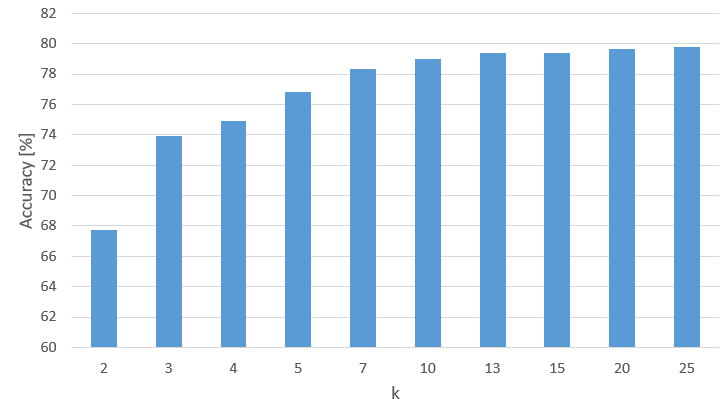
\includegraphics[width=0.9\textwidth]{accuracyK.png}
	\caption{Wykres przedstawiający zależność Accuracy od wartości k (dane treningowe/testowe 50\%/50\%, Metryka euklidesowa).}
	\label{accuracyK}
\end{figure}

\newpage
\subsection{Badanie wyników klasyfikacji w zależności od podziału na dane treningowe i testowe}
\begin{table}[h!]
	\centering
	\begin{tabular} {c c c c c c}
		\hline
		\textbf{Dane tren./test.} & \textbf{Accuracy [\%]} & \vline & \textbf{Place} & \textbf{Precision [\%]} & \textbf{Recall [\%]}\\ [0.5ex] 
		\hline 
		\hline 
		&   			&\vline& USA & 79,525 & 98,918 \\
		&				&\vline& CAN & 10,526 & 0,743 \\
		30/70 & 78,325  &\vline& FRA & 0,000 & 0,000 \\
		&				&\vline& JAP & 0,000 & 0,000 \\
    	&				&\vline& W-G & 0,000 & 0,000 \\
		&		 		&\vline& UK  & 12,500 & 0,963 \\
		\hline
		&   			&\vline& USA & 79,958 & 98,773 \\
		&				&\vline& CAN & 17,241 & 1,309 \\
		50/50 & 78,979  &\vline& FRA & 0,000 & 0,000 \\
		&				&\vline& JAP & 7,692 & 0,355 \\
		&				&\vline& W-G & 0,000 & 0,000 \\
		&		 		&\vline& UK  & 13,462 & 1,720 \\
		\hline
		&   			&\vline& USA & 81,839 & 98,522 \\
		&				&\vline& CAN & 10,000 & 0,439 \\
		70/30 & 81,409  &\vline& FRA & 0,000 & 0,000 \\
		&				&\vline& JAP & 9,091 & 0,599 \\
		&				&\vline& W-G & 50,000 & 1,042 \\
		&		 		&\vline& UK  & 13,333 & 3,030 \\
		\hline
		&   			&\vline& USA & 83,570 & 98,764 \\
		&				&\vline& CAN & 20,000 & 0,649 \\
		80/20 & 82,911  &\vline& FRA & 0,000 & 0,000 \\
		&				&\vline& JAP & 0,000 & 0,000 \\
		&				&\vline& W-G & 100,000 & 1,574 \\
		&		 		&\vline& UK  & 23,333 & 6,140 \\
		\hline
		&   			&\vline& USA & 84,634 & 98,846 \\
		&				&\vline& CAN & 25,000 & 0,952 \\
		85/15 & 83,667  &\vline& FRA & 0,000 & 0,000 \\
		&				&\vline& JAP & 0,000 & 0,000 \\
		&				&\vline& W-G & 100,000 & 2,500 \\
		&		 		&\vline& UK  & 11,111 & 2,740 \\
		\hline
		\hline
	\end{tabular}
	\caption{Zależność Accuracy od pięciu wartości proporcji podziału zbioru dla k=10, metryka uliczna. }
	\label{tabelaTT}
\end{table}

\begin{figure}[h!]
    \centering
    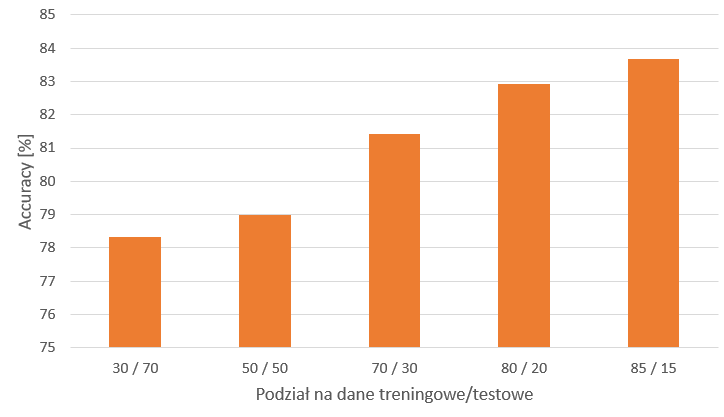
\includegraphics[width=1\textwidth]{accuracyTT.png}
    \caption{Wykres przedstawiający zależność Accuracy od pięciu wartości proporcji podziału zbioru, k=10, metryka uliczna.}
    \label{accuracyTT}
\end{figure}

\newpage
\subsection{Badanie zależności Accuracy od wyboru metryki}

\begin{table}[h!]
	\centering
	\begin{tabular} {c c c c c c}
		\hline
		\textbf{Metryka} & \textbf{Accuracy [\%]} & \vline & \textbf{Place} & \textbf{Precision [\%]} & \textbf{Recall [\%]}\\ [0.5ex] 
		\hline
		\hline
		&   					&\vline& USA & 81,918 & 99,457 \\
		&						&\vline& CAN & 25,000 & 0,439 \\
		euklidesowa & 81,409    &\vline& FRA & 0,000 & 0,000 \\
		&						&\vline& JAP & 0,000 & 0,000 \\
		&						&\vline& W-G & 0,000 & 0,000 \\
		&		 				&\vline& UK  & 25,000 & 3,535 \\
		\hline 
		&   					&\vline& USA & 81,900 & 99,337 \\
		&						&\vline& CAN & 40,000 & 0,877 \\
		Czebyszewa & 81,335     &\vline& FRA & 0,000 & 0,000 \\
		&						&\vline& JAP  & 0,000 & 0,000 \\
		&						&\vline& W-G & 0,000 & 0,000 \\
		&		 				&\vline& UK  & 25,000 & 3,535 \\
		\hline 
		&   					&\vline& USA & 81,816 & 99,457 \\
		&						&\vline& CAN & 100,000 & 0,877 \\
		uliczna & 81,384        &\vline& FRA & 0,000 & 0,000 \\
		&						&\vline& JAP & 33,333 & 0,599 \\
		&						&\vline& W-G & 0,000 & 0,000 \\
		&		 				&\vline& UK  & 16,000 & 2,020 \\
		\hline
		\hline
	\end{tabular}
	\caption{Zależność Accuracy od wyboru metryki dla k=13 i podziału 70/30. }
	\label{tabelaMetric}
\end{table}

\begin{figure}[h!]
    \centering
    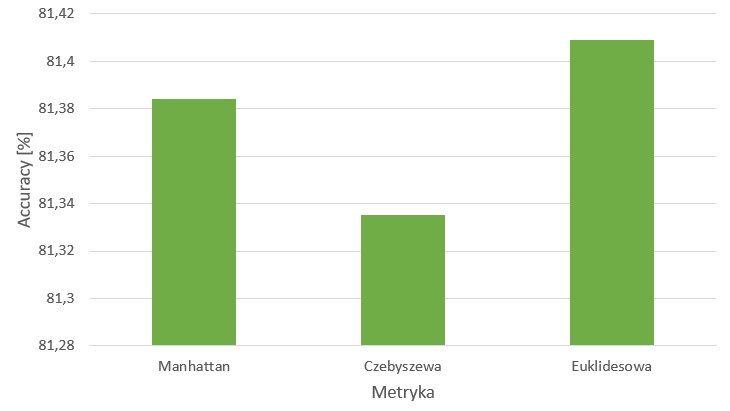
\includegraphics[width=1\textwidth]{accuracyMetric.png}
    \caption{Wykres przedstawiający zależność Accuracy od wyboru metryki dla k=13 i podziału 70/30.}
    \label{accuracyMetric}
\end{figure}

\newpage
\subsection{Badanie różnic w wyborze podzbioru cech}
\begin{table}[h!]
	\centering
	\begin{tabular} {c c c c c c}
		\hline
		\textbf{Podzbiór cech} & \textbf{Accuracy [\%]} & \vline & \textbf{Place} & \textbf{Precision [\%]} & \textbf{Recall [\%]}\\ [0.5ex] 
		\hline
		\hline 
		&   							&\vline& USA & 79,816 & 99,740 \\
		&								&\vline& CAN & 33,333 & 1,047 \\
		Wszystkie cechy & 79,573        &\vline& FRA & 0,000 & 0,000 \\
		&								&\vline& JAP & 0,000 & 0,000 \\
		&								&\vline& W-G & 0,000 & 0,000 \\
		&		 						&\vline& UK  & 0,000 & 0,000 \\
		\hline 
		&   										 	&\vline& USA & 79,81 & 100,000 \\
		&												&\vline& CAN & 0,000 & 0,000 \\
		$C_1, C_2, C_3, C_4, C_5, C_{11}$ & 79,81       &\vline& FRA & 0,000 & 0,000 \\
		&												&\vline& JAP & 0,000 & 0,000 \\
		&												&\vline& W-G & 0,000 & 0,000 \\
		&		 										&\vline& UK  & 0,000 & 0,000 \\
		\hline 
		&   											&\vline& USA & 79,863 & 99,591 \\
		&												&\vline& CAN & 22,222 & 0,524 \\
		$C_6, C_7, C_8, C_9, C_{10}$ & 79,558        	&\vline& FRA & 0,000 & 0,000 \\
		&												&\vline& JAP & 0,000 & 0,000 \\
		&												&\vline& W-G & 0,000 & 0,000 \\
		&		 										&\vline& UK  & 14,286 & 0,737 \\
		\hline 
		&   											&\vline& USA & 80,357 & 99,461 \\
		&												&\vline& CAN & 16,667 & 0,524 \\
		$C_1, C_2, C_3, C_8, C_9, C_{10}$ & 79,662      &\vline& FRA & 20,690 & 5,217 \\
		&												&\vline& JAP & 22,222 & 0,709 \\
		&												&\vline& W-G & 50,000 & 1,143 \\
		&		 										&\vline& UK  & 25,000 & 1,720 \\
		\hline 
		&   										&\vline& USA & 79,813 & 99,944 \\
		&											&\vline& CAN & 0,000 & 0,000 \\
		$C_4, C_5, C_6, C_7, C_{11}$ & 79,78        &\vline& FRA & 0,000 & 0,000 \\
		&											&\vline& JAP & 0,000 & 0,000 \\
		&											&\vline& W-G & 0,000 & 0,000 \\
		&		 									&\vline& UK  & 25,000 & 0,246 \\
		\hline 
		\hline
	\end{tabular}
	\caption{Zależność Accuracy od wyboru podzbioru cech dla k=20, podziału 50/50 i metryki Czebyszewa. }
	\label{tabelaFeatures}
\end{table}

\begin{figure}[h!]
    \centering
    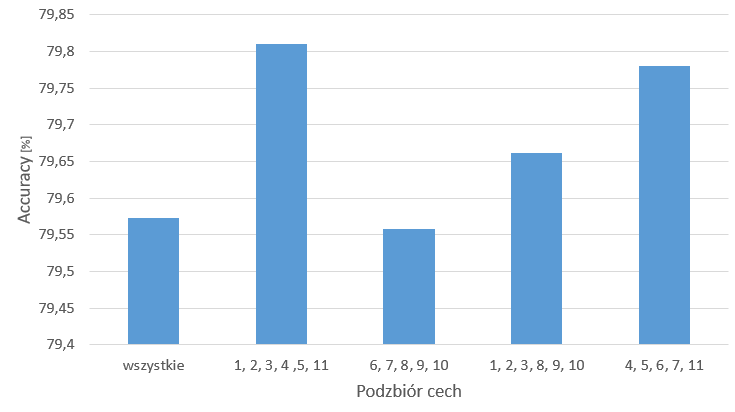
\includegraphics[width=1\textwidth]{accuracyFeatures.png}
    \caption{Wykres przedstawiający zależność Accuracy od wyboru podzbioru cech, k=20, podział 50/50, metryka Czebyszewa.}
    \label{accuracyFeatures}
\end{figure}

\newpage
\section{Dyskusja} % Dyskusja
\subsection{Wyniki klasyfikacji w zależności od parametru k}
Dobór odpowiedniej wartości parametru k ma duży wpływ na wynik klasyfikacji. Im większa wartość k, tym większa skuteczność klasyfikacji. Można to zauważyć na rysunku \ref{accuracyK}, jak i również tabeli \ref{tabelaK}. Największy skok widać między $k=2$ a $k=3$. Natomiast przy wartościach wyższych niż 10 różnica jest bardzo niewielka. Najlepsze wyniki klasyfikacji były osiągane, gdy $k=25$ - ok. 80\%, natomiast najgorsze, gdy $k=2$ - ok. 68\%.

Porównując miarę Recall na etykiecie USA można zauważyć, że rośnie ona wraz ze wzrostem k, natomiast Precision maleje. Dzieje się tak, ponieważ im większe zostało wybrane k, tym coraz więcej artykułów zostaje zakwalifikowanych jako USA - dla k = 25 dla etykiet $Canada, France, Japan$ oraz $West-Germany$ wyniki zarówno dla Recall oraz Precision wyniosły 0.
\subsection{Wyniki klasyfikacji w zależności od podziału na dane treningowe i testowe}
W przypadku podziału na dane testowe i treningowe, dla większej ilości danych treningowych algorytm był w stanie lepiej zaklasyfikować teksty i skuteczność klasyfikacji była wyższa. Dla badanych przez nas podziałów największą skuteczność osiągnął podział 85\% dane treningowe i 15\% dane testowe. Najgorsza jakość klasyfikacji została osiągnięta dla podziału 30\% treningowe / 70\% testowe. 

Analizując rysunek \ref{accuracyTT} oraz tabelę \ref{tabelaTT} największy skok wystąpił między podziałami 50/50 a 70/30. W przypadku tego drugiego podziału algorytm był w stanie się lepiej nauczyć.

Dla małej ilości danych treningowych dla etykiety $west-germany$ Precision i Recall wyniosło 0\%, a dla dużej ilości danych treningowych Precision wyniosło 100\%, a Recall 2,5\%. Dla pozostałych etykiet wyniki były do siebie zbliżone.
\subsection{Zależność Accuracy od wyboru metryki}
Wybór metryki w przypadku klasyfikowania artykułów wg kategorii \textsl{places} miał bardzo mały wpływ na wyniki klasyfikacji. Widać to na rysunku \ref{accuracyMetric}, a najlepiej w tabeli \ref{tabelaMetric}. Pomiędzy najlepszym wynikiem dla metryki euklidesowej, a najgorszym dla metryki Czebyszewa różnica była mniejsza niż 0.1 p.p. 

Wyniki Precision oraz Recall dla poszczególnych etykiet również są bardzo do siebie zbliżone, jednak np. w przypadku Canada dla metryki euklidesowej Precision wyniosło 25\%, a dla metryki ulicznej - 100\%. W przypadku algorytmu k-NN wybór metryki ma minimalny wpływ na wyniki klasyfikacji, jednak najlepszą metryką jest metryka euklidesowa.
\subsection{Różnice w wyborze podzbioru cech}
Jak można zauważyć na rysunku \ref{accuracyFeatures} oraz tabeli \ref{tabelaFeatures}, najlepszą wartość klasyfikacji (79.81\%) osiągnął podzbiór składający się z cech: $C_1, C_2, C_3, C_4, C_5, C_{11}$. Są to cechy zależne od słów kluczowych. Natomiast cechy niezależące od słów kluczowych, tj. $C_6, C_7, C_8, C_9, C_{10}$ osiągnęły wynik najgorszy (79.558\%). Dla wszystkich cech ten wynik był podobny do wyniku dla cech 6-10. Różnice w skuteczności są niewielkie, lecz zauważalne. 

Dla etykiet $France, Japan, West-Germany$ tylko w jednym przypadku wartości Precision i Recall nie wyniosły 0\% - był to przypadek testowy dla podzbioru cech: $C_6, C_7, C_8, C_9, C_{10}$.

\newpage
\section{Wnioski}
\begin{itemize}
	\item Liczba k sąsiadów ma spory wpływ na skuteczność klasyfikacji. Jednakże, zmiana metryki, bądź podziału na dane testowe i treningowe również ma wpływ na wynik klasyfikacji.
	\item Im większe k, tym więcej artykułów zostanie przypisanych do klasy dominującej.
	\item Również istotny jest podział artykułów na dane testowe i treningowe zarówno dla Accuracy, jak i Precision i Recall. 
	\item W przypadku zbyt małej ilości danych treningowych wystąpi zjawisko niedouczenia.
	\item W przypadku zbyt dużej ilości danych treningowych wystąpi zjawisko przeuczenia.
	\item Wybór metryki ma minimalny, bliski zeru wpływ na wyniki klasyfikacji.
	\item Wartość Accuracy jest największa dla cech, które zależą od słów kluczowych.

\end{itemize}


\begin{thebibliography} {0}
\bibitem{anbook} Niewiadomski, Adam. Methods for the Linguistic Summarization of Data: Applications of Fuzzy Sets and Their Extensions. Akademicka Oficyna Wydawnicza EXIT. Warszawa, 2008. ISBN 978-83-60434-40-6
\bibitem{norm} Ciaburro, Giuseppe. Regression Analysis with R. Packt Publishing, 2018. ISBN 978-1-78862-730-6
\bibitem{wyklad} \textsl{https://ftims.edu.p.lodz.pl/pluginfile.php/132368/mod\_folder/content/0/
ksr-wyklad-2009.pdf?forcedownload=1} [dostęp 22.03.2020]
\bibitem{manh} \textsl{https://en.wikipedia.org/wiki/Taxicab\_geometry} [dostęp 01.04.2020]
\bibitem{cze} \textsl{https://en.wikipedia.org/wiki/Chebyshev\_distance} [dostęp 01.04.2020]
\bibitem{euc} \textsl{https://en.wikipedia.org/wiki/Euclidean\_distance} [dostęp 01.04.2020]
\bibitem{stemmer} \textsl{https://tartarus.org/martin/PorterStemmer/csharp.txt} [dostęp 22.03.2020]
\bibitem{stopword} \textsl{https://www.dotnetperls.com/stopword-dictionary} [dostęp 22.03.2020]
\bibitem{leniwy} \textsl{http://home.agh.edu.pl/~horzyk/lectures/miw/KNN.pdf} [dostęp 22.03.2020]
\bibitem{apr} \textsl{https://pl.wikipedia.org/wiki/Tablica\_pomy\%C5\%82ek} [dostęp 01.04.2020]

\end{thebibliography}
\end{document}